\section{Network definition}

Let's consider a Siamese network with two branches labelled $\A$ and $\B$, and a final layer that computes an inner product followed by a learned gain and bias.
The network is defined:
\begin{align}
\obj{y}_{i}^{s} & = \obj{W}_{i} \obj{x}_{i - 1}^{s} + \obj{b}_{i} && s = \A, \B; \quad i = 1, \dots, L\\
\obj{x}_{i}^{s} & = \sigma(\obj{y}_{i}^{s}) && s = \A, \B; \quad i = 1, \dots, L - 1 \\
u & = \langle \obj{y}_{L}^{\A}, \obj{y}_{L}^{\B} \rangle \\
y_{L+1} & = w_{L+1} u + b_{L+1}
\end{align}
with a final loss $\ell = E(y_{L + 1}) = f(\obj{x}_{0}^\A, \obj{x}_{0}^\B, \mathbf{W}, \mathbf{b})$.
The gradients for the final layers are:
\begin{align}
\grad{u} & = \grad{y}_{L+1} w_{L+1} \\
\grad{w}_{L+1} & = \grad{y}_{L+1} u \\
\grad{b}_{L+1} & = \grad{y}_{L+1} \\
\gradobj{y}_{L}^{\A} & = \grad{u} \obj{y}_{L}^{\B} = \grad{y}_{L+1} w_{L+1} \obj{y}_{L}^{\B} \\
\gradobj{y}_{L}^{\B} & = \grad{u} \obj{y}_{L}^{\A} = \grad{y}_{L+1} w_{L+1} \obj{y}_{L}^{\A}
\end{align}
The gradients for layers $1, \dots, L$ will be largely the same, except that the gradients for the weights $\gradobj{W}_{i}$ will be accumulated from both branches:
\begin{align}
\gradobj{W}_{i} & = \textstyle \sum_{s} \gradobj{y}_{i}^{s} (\obj{x}_{i - 1}^{s})^T && i = L, \dots, 1 \\
\gradobj{b}_{i} & = \textstyle \sum_{s} \gradobj{y}_{i}^{s} && i = L, \dots, 1 \\
\gradobj{x}_{i}^{s} & = \obj{W}_{i + 1}^T \gradobj{y}_{i + 1}^{s} && i = L-1, \dots, 1 \\
\gradobj{y}_{i}^{s} & = \nabla\sigma(\obj{y}_{i}^{s}) \odot \gradobj{x}_{i}^{s} && i = L - 1, \dots, 1
\end{align}

It can be seen that the gradients $\gradobj{y}_{L}^{s}$ are now scaled by $w_{L+1}$ and $\obj{y}_{L}^{t}$ where $t \ne s$.
This is quite different to what we saw before, since the gradients of the activations $\gradobj{y}_{L}^{s}$ are scaled by the activations themselves $\obj{y}_{L}^{t}$.


\section{Analysis}

\subsection{Magnitude of output}

Assume that $\obj{b}_{i} = 0$.
As before:
\begin{align}
\E[y_{i}] & = 0 \\
\V[y_{i}] & = m_{i - 1} \V[W_{i}] \E[x_{i - 1}^2] \\ % && i = 1, \dots, L \\
\E[x_{i}^2] % & = \tfrac{1}{2} \V[y_{i}] \nonumber \\
& = \tfrac{1}{2} m_{i - 1} \V[W_{i}] \E[x_{i - 1}^2] % && i = 1, \dots, L-1
\end{align}

The first thing to consider is the magnitude of the output $y_{L+1}$.
It is not clear whether we can assume that $\obj{y}_{L}^{\A}$ and $\obj{y}_{L}^{\B}$ are independent in
\begin{equation}
u = \langle \obj{y}_{L}^{\A}, \obj{y}_{L}^{\B} \rangle
= \sum_{k = 1}^{m_{L}} (\obj{y}_{L}^{\A})_{k} (\obj{y}_{L}^{\B})_{k}
\end{equation}
Let's consider two cases: one which assumes that they are independent:
\begin{align}
\E_{\bot}[u] & = m_{L} \E_{\bot}[y_{L}^{\A} \cdot y_{L}^{\B}] \\
& = m_{L} \E[y_{L}^{\A}] \E[y_{L}^{\B}] \\
& = m_{L} \E[y_{L}]^2 \qquad \text{since $\E[y_{L}] = 0$} \\
& = 0 \\
\V_{\bot}[u] & = m_{L} \V_{\bot}[y_{L}^{\A} \cdot y_{L}^{\B}] \\
& = m_{L} \left( \E[y_{L}^2] \E[y_{L}^2] - \E[y_{L}]^2 \E[y_{L}]^2 \right) \\
& = m_{L} \V[y_{L}]^2 \qquad \text{since $\E[y_{L}] = 0$} \\
\intertext{and one which assumes they are equal:}
\E_{\parallel}[u]
& = m_{L} \E_{\parallel}[y_{L}^{\A} \cdot y_{L}^{\B}] \approx m_{L} \E[y_{L}^2] \\
& = m_{L} \V[y_{L}] \\
\V_{\parallel}[u]
& = m_{L} \V_{\parallel}[y_{L}^{\A} \cdot y_{L}^{\B}] \approx m_{L} \V[y_{L}^2] \\
& \approx 2 m_{L} \V[y_{L}]^2
%\E_{\parallel}[u^2] & \approx 3 m_{L} \V[y_{L}]^2
\end{align}
where we have assumed that $y_{L}$ is approximately Gaussian and therefore has kurtosis $\E[y_{L}^4] \approx 3 \V[y_L]^2$ and $\V[y_{L}^2] \approx 2 \V[y_L]^2$.
Note that the assumption made has a much bigger effect on the mean (which becomes non-zero) than the variance (which roughly doubles).

The result above is concerning because the variance of the inner product is the square of the variance of the embedding.
Perhaps we should try to achieve $\V[y_{L}] \approx 1$ to limit the effect.

Finally, let's examine the output.
Consider $w_{L+1}$ and $b_{L+1}$ to be simple scalars rather than random variables.
\begin{align}
\E[y_{L+1}]
& = \E[w_{L+1} u] + \E[b_{L+1}] \\
& = w_{L+1} \E[u] + b_{L+1} \\
%& = m_{L} w_{L+1} \V[y_{L}] + b_{L+1} = 0 \\
\V[y_{L+1}]
& = \V[w_{L+1} u] + b_{L+1} \\
& = w_{L+1}^2 \V[u]
%& \approx 2 m_{L} w_{L+1}^2 \V[y_{L}]^2
\end{align}

%Note that, to achieve $\E[y_{L+1}] = 0$, we choose $b_{L+1} = -m_{L} w_{L+1} \V[y_{L}]$.

\subsection{Magnitude of gradients}

As before:
\begin{align}
\V[\grad{x}_{i}] & = m_{i+1} \V[W_{i+1}] \V[\grad{y}_{i+1}] \\
\V[\grad{y}_{i}] & = \tfrac{1}{2} m_{i+1} \V[W_{i+1}] \V[\grad{y}_{i+1}]
\end{align}
For the parameters in the branches, we must accumulate gradients from both
\begin{align}
\V[\grad{W}_{i}] & = 2 \V[\grad{y}_{i}] \E[x_{i-1}^2] \\
\V[\grad{b}_{i}] & = 2 \V[\grad{y}_{i}]
\end{align}

Let's inspect the gradients of the output subnet, assuming that $\E[\grad{y}_{L+1}] = 0$
\begin{align}
%\grad{u} & = \grad{y}_{L+1} w_{L+1} \\
\E[\grad{u}]
& = \E[\grad{y}_{L+1} w_{L+1}] \\
& = w_{L+1} \E[\grad{y}_{L+1}] = 0 \\
\E[\grad{y}_{L}] & = \E[\grad{u} y_{L}] \\
& = \E[\grad{u}] \E[y_{L}] = 0
\end{align}
\begin{align}
\V[\grad{u}]
& = \V[\grad{y}_{L+1} w_{L+1}] \\
& = w_{L+1}^2 \V[\grad{y}_{L+1}] \\
%& = \E[\grad{y}_{L+1}^2] \E[w_{L+1}^2] - \E[\grad{y}_{L+1}]^2 \E[w_{L+1}]^2 \\
%& = \V[\grad{y}_{L+1}] \E[w_{L+1}^2] \\
\V[\grad{y}_{L}]
& = \V[\grad{u} y_{L}] \\
& = \E[\grad{u}^2] \E[y_{L}^2] - \E[\grad{u}]^2 \E[y_{L}]^2 \\
& = \V[\grad{u}] \V[y_{L}] \\
& = w_{L+1}^2 \V[y_{L}] \V[\grad{y}_{L+1}]
\end{align}
\begin{align}
\E[\grad{b}_{L+1}] & = \E[\grad{y}_{L+1}] = 0 \\
\V[\grad{b}_{L+1}] & = \V[\grad{y}_{L+1}] = 0 \\
\E[\grad{w}_{L+1}]
& = \E[\grad{y}_{L+1} u] \\
& = \E[\grad{y}_{L+1}] \E[u] = 0 \qquad \text{since $\E[\grad{y}_{L+1}] = 0$} \\
\V[\grad{w}_{L+1}]
& = \V[\grad{y}_{L+1} u] \\
& = \E[\grad{y}_{L+1}^2] \E[u^2] - \E[\grad{y}_{L+1}]^2 \E[u]^2 \\
& = \V[\grad{y}_{L+1}] \E[u^2] \qquad \text{since $\E[\grad{y}_{L+1}] = 0$}
%& = 3 m_{L} \V[y_{L}]^2 \V[\grad{y}_{L+1}]
\end{align}
The term $\V[y_{L}]^2$ has also appeared in the magnitude of the gradients.

%\begin{align}
%\V[\grad{y}_{L}]
%& = \V[\grad{y}_{L+1}] \E[w_{L+1}^2] \V[y_{L}] \\
%& = \V[\grad{y}_{L+1}] \E[w_{L+1}^2] \cdot m_{i - 1} \V[W_{i}] \E[x_{i - 1}^2] \\
%\end{align}

%Compare this to the other weights' gradients
%\begin{align}
%\V[\grad{W}_{i}] & = 2 \V[\grad{y}_{i}] \E[x_{i - 1}^2] && i = 1, \dots, L
%\end{align}
%Whereas the former is a product of three variances, the latter is a product of two variances (or variance-like values).
%Assuming that the magnitude of these variances are similar, we should aim to keep $\V[y_{L}] \approx 1$, or else the magnitude of the grad $\V[\grad{w}_{L+1}]$ may be significantly different to other magnitudes.

%How can we influence $\V[y_{L}]$?
%\begin{align}
%\V[y_{L}] & = 2 \left(\prod_{j = 1}^{i} \tfrac{1}{2} m_{j - 1} \V[W_{j}]\right) \E[x_{0}^2] \\
%\intertext{assume $\E[x_{0}^2] = 1$}
%\V[y_{L}] & = 2 \left(\prod_{j = 1}^{L} \tfrac{1}{2} m_{j - 1} \alpha_{j}^2\right) \\
%\intertext{and if we adopt $\alpha_{j}^2 = 2/m_{j}$ for $j \ge 2$}
%\V[y_{L}] & = m_{0} \alpha_{1}^2 \left(\prod_{j = 2}^{L} \frac{m_{j-1}}{m_{j}} \right)
%  = \frac{m_{0} m_{1} \alpha_{1}^2}{m_{L}}
%\end{align}
%Therefore we can choose
%\begin{equation}
%\alpha_{1}^2 = \frac{m_{L}}{m_{0} m_{1}}
%\end{equation}
%to achieve $\V[y_{L}] = 1$.
%If we assume that all $m_{i}$ are roughly equal, we could use $\alpha_{i}^2 = 1 / \sqrt{m_{0} m_{1}}$.
%\begin{align}
%\V[\grad{w}_{L+1}] = m_{L} \V[\grad{y}_{L+1}] \V[y_{L}]^{2}
%\end{align}
%
%We still observe a big difference between $\V[\grad{w}_{L+1}]$ and $\V[\grad{W}_{i}]$.
%Note that also the magnitude of $\grad{w}_{L+1} \approx 1$ is 
%
%We also need the initial output to be of the desired magnitude.
%How can we control the magnitude of the 


\subsection{Equal-magnitude activations}

Recall that it was possible to achieve $\V[y_{i}] = \V[y_{i-1}]$ and therefore $\V[y_{L}] = 2 \E[x_{0}^2]$ by choosing $\V[W_{i}] = 2 / m_{i}$ for all $i$.
For the rest of this section, we consider the specific case $\V[W_{i}] = 2 / m_{i-1}$ for $i = 1, \dots L$ and further assume that $\E[x_{0}^{2}] = 1$ to simplify the expressions.
This provides $\V[y_{L}] = 2 \E[x_{0}^2] = 2$.

How should we choose $w_{L+1}^2$ and $b_{L+1}$ to achieve $\E[y_{L+1}] = 0$ and $\V[y_{L+1}] = \V[y_{L}]$?
If we adopt the assumption that $\obj{y}_{\A}$ and $\obj{y}_{\B}$ are independent, then we obtain:
\begin{align}
0 = \E[y_{L+1}] & = w_{L+1} \E_{\bot}[u] + b_{L+1} = b_{L+1} \\
b_{L+1} & = 0
\end{align}
\begin{align}
\V[y_{L}] = \V[y_{L+1}] & = w_{L+1}^2 \V_{\bot}[u] = m_{L} w_{L+1}^2 \V[y_{L}]^2 \\
1 & = m_{L} w_{L+1}^2 \V[y_{L}] \\
w_{L+1}^2 & = 1 / (m_{L} \V[y_{L}]) = 1 / (2 m_{L})
\end{align}
If we instead assume that $\obj{y}_{\A} = \obj{y}_{\B}$, then we obtain:
\begin{align}
0 = \E[y_{L+1}] & = w_{L+1} \E_{\parallel}[u] + b_{L+1} = m_{L} w_{L+1} \V[y_{L}] + b_{L+1} \\
b_{L+1} & = -m_{L} w_{L+1} \V[y_{L}] = -2 m_{L} w_{L+1}
\end{align}
\begin{align}
\V[y_{L}] = \V[y_{L+1}] & = w_{L+1}^2 \V_{\parallel}[u] = 2 m_{L} w_{L+1}^2 \V[y_{L}]^2 \\
1 & = 2 m_{L} w_{L+1}^2 \V[y_{L}] \\
w_{L+1}^2 & = 1 / (2 m_{L} \V[y_{L}]) = 1 / (4 m_{L})
\end{align}
Happily, in either case this implies that $\V[W_{i}]$ and $w_{L+1}^2$ are approximately equal (within an order of magnitude).

We might instead choose $w_{L} = 1 / m_{L}$ (that is, $w_{L}^2 = 1 / m_{L}^2$) to remove the dependence of $\E[y_{L}]$ on $m_{L}$.
Unfortunately this makes $w_{L}^2$ different to $\V[W_{i}]$ by a factor of $m$ (at least $w_{L}$ and $\operatorname{std}[W_{i}]$ only differ by a factor of $\sqrt{m}$).
Under the assumption that the two branches are equal, this leads to
\begin{align}
\E[y_{L+1}] & = m_{L} w_{L+1} \V[y_{L}] + b_{L+1} \\
& = 2 - b_{L+1}
\end{align}
\begin{align}
\V[y_{L+1}] & = 2 m_{L} w_{L+1}^2 \V[y_{L}]^2 \\
& = 4 m_{L} (1 / m_{L}^2) \\
& = 4 / m_{L}
\end{align}
Note that this only implies $\std[y_{L+1}] \propto 1 / \sqrt{m_{L}}$.
% As a middle ground, we might consider $w_{L} = m_{L}^{-3/4}$.

Is this different from multiplying the dot product by a constant $1 / m_{L}$ in terms of gradients?
What about pre-multiplying both branches by $1 / \sqrt{m_L}$?

%Recall that choosing $\V[W_{i}] = 2 / m_{i}$ for all $i$ was sufficient to ensure that $\V[y_{i}] = \V[y_{i-1}]$ and therefore $\V[y_{L}] = 2 \E[x_{0}^2]$.
%%(It might be possible to eliminate this factor of $2$ using a factor of $2^{\frac{1}{L}}$ at each layer.)
%%Let us entertain this scenario, and further assume that $\E[x_{0}^2]$.

%Recall that expanding the recursions for $\V[\grad{y}_{i}]$ and $\E[x_{i-1}^2]$ gives
%\begin{align}
%\V[\grad{W}_{i}] = \frac{C}{m_{i-1} m_{i} \V[W_{i}]}
%\end{align}
%where
%\begin{equation}
%C = \frac{1}{2^{L-1}} \left(\prod_{j=0}^{L} m_{j} \right) \left(\prod_{j=1}^{L} \V[W_{j}] \right)
%  \E[x_{0}^2] \V[\grad{y}_{L}]
%\end{equation}
%If we similarly substitute in the expression for $\V[y_{L}]$:
%\begin{align}
%\V[\grad{w}_{L+1}]
%& = m_{L} \V[\grad{y}_{L+1}] \V[y_{L}]^{2} \\
%& = m_{L} \V[\grad{y}_{L+1}] \left\{
%  2 \left( \prod_{j = 1}^{i} \tfrac{1}{2} m_{j - 1} \V[W_{j}] \right) \E[x_{0}^2] \right\}^2 \\
%& = 2^2 m_{L} \V[\grad{y}_{L+1}] \left( \prod_{j = 1}^{i} \tfrac{1}{2^2} m_{j - 1} \V[W_{j}]^2 \right) \E[x_{0}^2]^2 \\
%\end{align}
%This does not look promising.

%Then, to achieve $\V[y_{L+1}] = \V[y_{L}] = 2$, we should choose
%\begin{align}
%w_{L+1}^2 & = \frac{1}{2 m_{L} \V[y_{L}]} = \frac{1}{4 m_{L}} \\
%%b_{L+1} & = -m_{L} w_{L+1} \V[y_{L}] = -m_{L} \cdot \frac{1}{2 \sqrt{m_{L}}} \cdot 2 = -\sqrt{m_{L}}
%b_{L+1} & = -m_{L} w_{L+1} \V[y_{L}] = -2 m_{L} w_{L+1}
%\end{align}
%This implies that $\V[W_{i}] = 1 / m_{i} \approx 1 / (4 m_{L}) = w_{L+1}^2$ are approximately equal (within an order of magnitude).

The figure below shows the outcome of assuming the weights are independent or equal.

\begin{figure}[H]
\centering
\begin{tabular}{c @{} c @{} c}
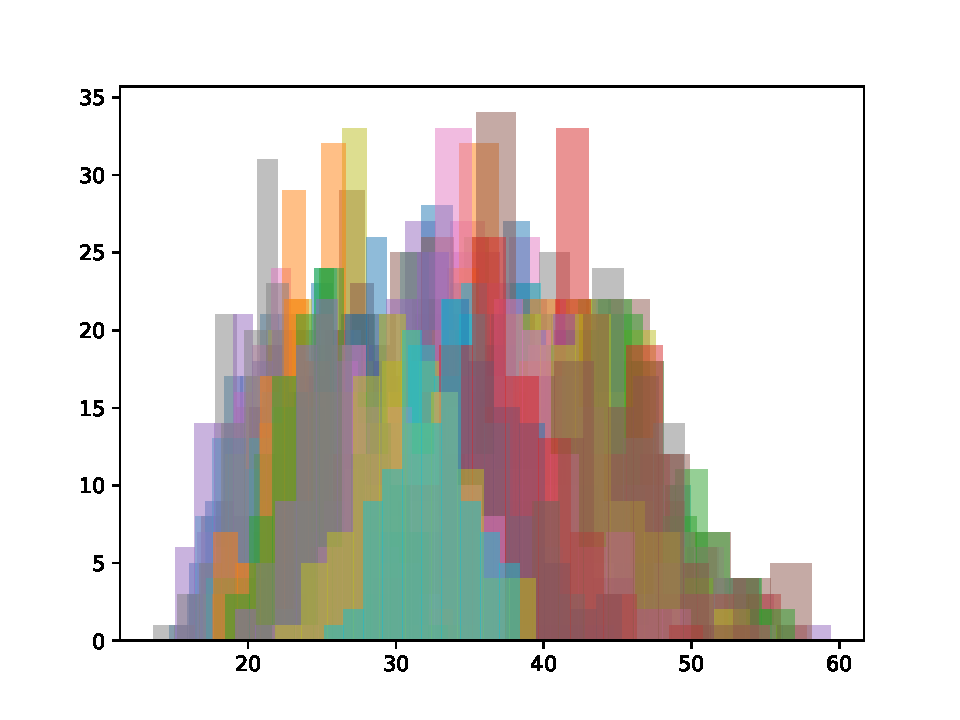
\includegraphics[width=40mm]{figures/siamese_hist_independent} &
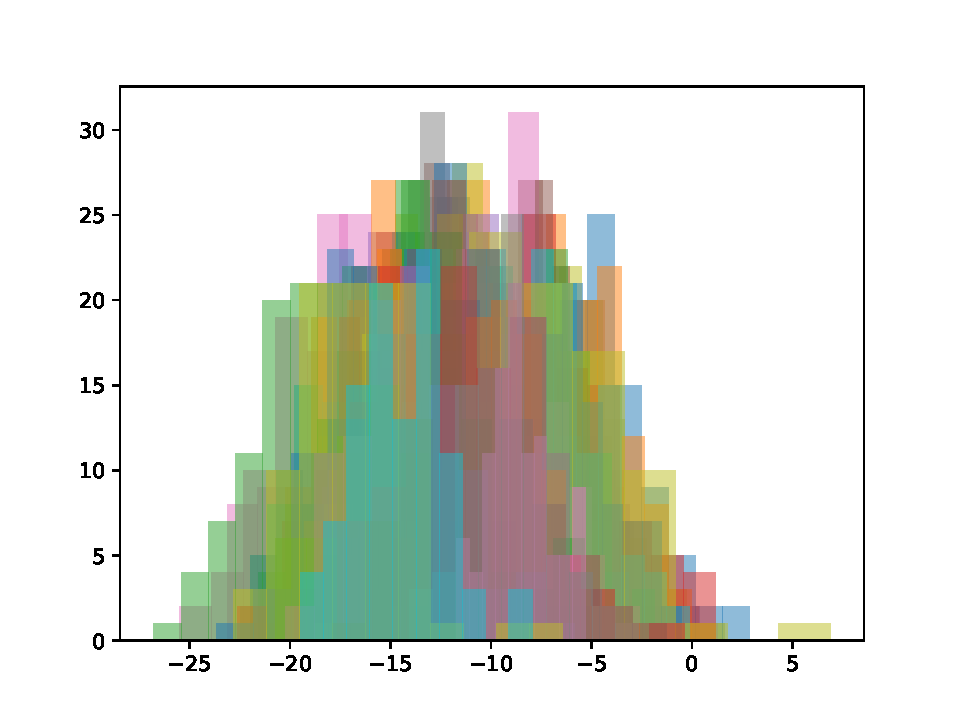
\includegraphics[width=40mm]{figures/siamese_hist_equal} &
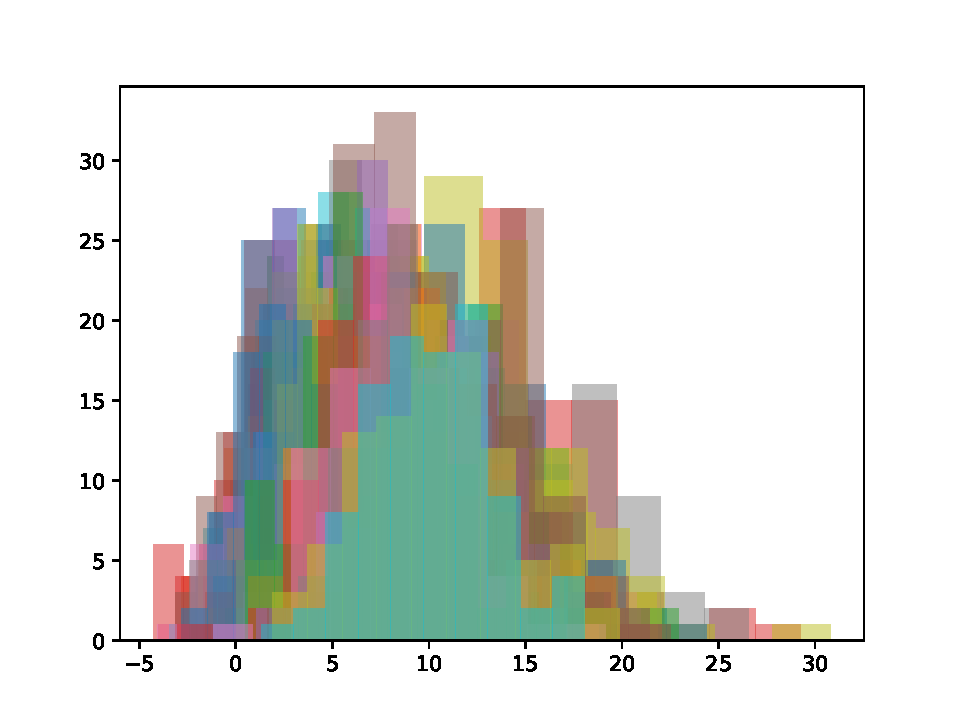
\includegraphics[width=40mm]{figures/siamese_hist_compromise} \\
(a) assume independent &
(b) assume equal &
(c) compromise \\
\end{tabular}
\caption{
  The output distribution of $y_{L}$.
  Each color shows the distribution of outputs obtained with random inputs for a fixed network.
}
\end{figure}

Could we fix the bias by computing the sample mean and initializing an extra parameter?
This sounds similar to batch-norm, except the mean would only be used as initialization.

Important remark: The analysis is greatly complicated by the fact that the activations from the two branches are not independent.
We lose the zero-mean assumption for the network output.
Maybe we should focus on the use of batch-norm?

We would not have this problem if we used the difference between two embeddings!

TODO: From here onwards may be invalidated due to incorrect assumption that $\obj{y}_{L}^{\A}$ and $\obj{y}_{L}^{\B}$ are independent.

Now let's consider the effect of the choice of $\V[W_{i}]$, $w_{L+1}^2$ and $b_{L+1}$ on the gradients.
\begin{align}
\V[\grad{W}_{i}]
& = \frac{2 C}{m_{i-1} m_{i} \V[W_{i}]} \\
C & = \frac{1}{2^{L-1}} \left(\prod_{j=0}^{L} m_{j} \right) \left(\prod_{j=1}^{L} \frac{2}{m_{j}} \right)
  \E[x_{0}^2] \V[\grad{y}_{L}] \\
& = 2 m_{0} \V[\grad{y}_{L}] \\
\V[\grad{W}_{i}]
%& = \frac{2 C}{m_{i-1} m_{i} \V[W_{i}]} \\
& = \frac{2 \cdot 2 m_{0}}{m_{i-1} m_{i} (2 / m_{i})} \V[\grad{y}_{L}] \\
& = \frac{2 m_{0}}{m_{i-1}} \V[\grad{y}_{L}] \\
& = \frac{m_{0}}{m_{i-1}} \E[w_{L+1}^2] \V[y_{L}] \V[\grad{y}_{L+1}] \\
%& = \frac{m_{0}}{m_{i-1}} \frac{1}{2 m_{L}} (2^2) \V[\grad{y}_{L+1}] \\
& = \frac{2 m_{0}}{m_{i-1} m_{L}} \V[\grad{y}_{L+1}] \\
\V[\grad{w}_{L+1}]
& = m_{L} \V[y_{L}]^{2} \V[\grad{y}_{L+1}] \\
& = 2^2 m_{L} \V[\grad{y}_{L+1}]
\end{align}
This shows that $\V[\grad{W}_{i}] \propto 1/m_{L}$, whereas $\V[\grad{w}_{L+1}] \propto m_{L}$, where $m_{L}$ is the dimension of the embedding.
This is a relative difference of $m_{L}^2$ between the variances ($m_{L}$ between the root-variances).
Recall that the magnitudes of the parameters are similar.

The $1/m_{L}$ term in $\V[\grad{w}_{L+1}]$ arose due to the need to choose $\E[w_{L+1}^2] \propto m_{L}^{-1}$ in order to obtain a suitable output magnitude $\V[y_{L+1}] \approx 1$.

%And the gradients for the bias terms?
%\begin{align}
%\V[\grad{b}_{i}] & =  \\
%\V[\grad{b}_{L+1}] & = 
%\end{align}

One solution may simply be to adopt different learning rates.
For example, if we choose $\lambda_{w_{L+1}} = (1 / m_{L}) \lambda$.

Would different choices of $\V[W_{i}]$ be better?
Perhaps we can introduce a global scale parameter $\alpha^2$ that effects $\V[y_{L+1}] \approx 1$ without $\E[w_{L+1}^2] \propto m_{L}^{-1}$?

Maybe we could alternatively achieve $\V[y_{L+1}] \approx 1$ by multiplying the inner product by a constant?
Is this equivalent to a re-parameterization of $w_{L+1}$ and therefore simply adjusting the learning rate?

Or maybe we can achieve $\V[y_{L+1}] \approx 1$ by introducing batch-norm before or after the inner product?


\clearpage

\subsection{Magnitude of gradients}

Let's inspect the gradients of the output subnet (assuming that $\E[\grad{y}_{L+1}] = 0$ and $\E[y_{L}] = 0$)
\begin{align}
\V[\grad{w}_{L+1}] = m_{L} \V[\grad{y}_{L+1}] \V[y_{L}]^{2}
\end{align}
Compare this to the other weights' gradients
\begin{align}
\V[\grad{W}_{i}] & = 2 \V[\grad{y}_{i}] \E[x_{i - 1}^2] && i = 1, \dots, L
\end{align}
Whereas the former is a product of three variances, the latter is a product of two variances (or variance-like values).
Assuming that the magnitude of these variances are similar, we should aim to keep $\V[y_{L}] \approx 1$, or else the magnitude of the grad $\V[\grad{w}_{L+1}]$ may be significantly different to other magnitudes.

How can we influence $\V[y_{L}]$?
\begin{align}
\V[y_{L}] & = 2 \left(\prod_{j = 1}^{i} \tfrac{1}{2} m_{j - 1} \V[W_{j}]\right) \E[x_{0}^2] \\
\intertext{assume $\E[x_{0}^2] = 1$}
\V[y_{L}] & = 2 \left(\prod_{j = 1}^{L} \tfrac{1}{2} m_{j - 1} \alpha_{j}^2\right) \\
\intertext{and if we adopt $\alpha_{j}^2 = 2/m_{j}$ for $j \ge 2$}
\V[y_{L}] & = m_{0} \alpha_{1}^2 \left(\prod_{j = 2}^{L} \frac{m_{j-1}}{m_{j}} \right)
  = \frac{m_{0} m_{1} \alpha_{1}^2}{m_{L}}
\end{align}
Therefore we can choose
\begin{equation}
\alpha_{1}^2 = \frac{m_{L}}{m_{0} m_{1}}
\end{equation}
to achieve $\V[y_{L}] = 1$.
If we assume that all $m_{i}$ are roughly equal, we could use $\alpha_{i}^2 = 1 / \sqrt{m_{0} m_{1}}$.
\begin{align}
\V[\grad{w}_{L+1}] = m_{L} \V[\grad{y}_{L+1}] \V[y_{L}]^{2}
\end{align}

We still observe a big difference between $\V[\grad{w}_{L+1}]$ and $\V[\grad{W}_{i}]$.
Note that also the magnitude of $\grad{w}_{L+1} \approx 1$ is 

We also need the initial output to be of the desired magnitude.
How can we control the magnitude of the 

\vspace{2em}

Additionally, we might also want to consider the dot product normalized by the square root of the number of elements
\begin{equation}
h(x, y) = \frac{1}{\sqrt{m}} \sum_{i = 1}^{m} \obj{x}_{i} \obj{y}_{i}
\end{equation}
Let us introduce a constant $\rho$ that controls the magnitude of the inner product
\begin{equation}
y_{L+1} = w_{L+1} \cdot \rho \cdot \langle \obj{y}_{L}^{\A},  \obj{y}_{L}^{\B} \rangle + b_{L+1}
\end{equation}
which affects the local gradients at the output:
\begin{equation}
\left\{ \begin{aligned}
\grad{w}_{L+1} & = \grad{y}_{L+1} \rho \langle \obj{y}_{L}^{\A}, \obj{y}_{L}^{\B} \rangle \\
\gradobj{y}_{L}^{\A} & = \grad{y}_{L+1} \rho w_{L+1} \obj{y}_{L}^{\B} \\
\gradobj{y}_{L}^{\B} & = \grad{y}_{L+1} \rho w_{L+1} \obj{y}_{L}^{\A}
\end{aligned} \right.
\end{equation}
This will scale all gradients in the network by $\rho$ without affecting the magnitude of the weights $\V[W_{i}]$.

If we are hypothesizing that the important thing is the \emph{relative} magnitude of the grad, maybe we can use this to adjust the relative magnitudes of all weights?
But would it also place an initial prior on the weights?
Maybe we can periodically re-parameterize the network to achieve the desired properties?

The magnitudes of the modified gradients are
\begin{align}
\V[\grad{w}_{L+1}] = \rho^{2} m_{L} \V[\grad{y}_{L+1}] \V[y_{L}]^{2}
\end{align}
If we set $\rho = \sqrt{m_{L}}$, we should be able to achieve $\V[\grad{w}_{L+1}] = 1$.


%\begin{align}
%f(\obj{x}_{0}^\A, \obj{x}_{0}^\B, \obj{W}_{1 \dots L+1}, \obj{b}_{1 \dots L+1})
%& = f_{i}(\obj{x}_{i}^\A, \obj{x}_{i}^\B, \obj{W}_{i+1 \dots L+1}, \obj{b}_{i+1 \dots L+1})
%\end{align}
%\begin{align}
%\langle \gradobj{y}_{L+1}, dy_{L+1} \rangle
%& = \langle \gradobj{x}_{L+1}, dy_{L+1} \rangle
%& = f_{i}(\obj{x}_{i}^\A, \obj{x}_{i}^\B, \obj{W}_{i+1 \dots L+1}, \obj{b}_{i+1 \dots L+1})
%\end{align}

\begin{subappendices}

\section{Gradients}

Let $u = \langle \obj{y}_{L}^{\A}, \obj{y}_{L}^{\B} \rangle$ such that $y_{L+1} = w_{L+1} u + b_{L+1}$.
The differentials are
\begin{equation}
\left\{ \begin{aligned}
dy_{L+1} & = dw_{L+1} u + w_{L+1} du + db_{L+1} \\
du & = \langle \obj{dy}_{L}^{\A}, \obj{y}_{L}^{\B} \rangle + \langle \obj{y}_{L}^{\A}, \obj{dy}_{L}^{\B} \rangle
\end{aligned} \right.
\end{equation}
Obtaining the gradients:
%\begin{align}
%\gradobj{y}_{L+1} dy_{L+1}
%& = \gradobj{y}_{L+1} \left(dW_{L+1} u + \obj{W}_{L+1} du + db_{L+1}\right) \\
%& = \gradobj{y}_{L+1} \left(dW_{L+1} u + \obj{W}_{L+1} du + db_{L+1}\right) \\
%& = \gradobj{W}_{L+1} dW_{L+1} + \grad{u} du + \gradobj{b}_{L+1} db_{L+1}
%\end{align}
\begin{equation}
\left\{ \begin{aligned}
\grad{u} & = \grad{y}_{L+1} w_{L+1} \\
\grad{w}_{L+1} & = \grad{y}_{L+1} u = \grad{y}_{L+1} \langle \obj{y}_{L}^{\A}, \obj{y}_{L}^{\B} \rangle \\
\grad{b}_{L+1} & = \grad{y}_{L+1}
\end{aligned} \right.
\end{equation}
and:
%\begin{align}
%\grad{u} du
%& = \grad{u} \left( \langle dy_{L}^{\A},  \obj{y}_{L}^{\B} \rangle + \langle \obj{y}_{L}^{\A},  dy_{L}^{\B} \rangle \right) \\
%& = \grad{u} \left( \langle dy_{L}^{\A},  \obj{y}_{L}^{\B} \rangle + \langle \obj{y}_{L}^{\A},  dy_{L}^{\B} \rangle \right) \\
%& = \langle \gradobj{y}_{L}^{\A}, dy_{L}^{\A} \rangle + \langle \gradobj{y}_{L}^{\B}, dy_{L}^{\B} \rangle
%\end{align}
\begin{equation}
\left\{ \begin{aligned}
\gradobj{y}_{L}^{\A} & = \grad{u} \obj{y}_{L}^{\B} = \grad{y}_{L+1} w_{L+1} \obj{y}_{L}^{\B} \\
\gradobj{y}_{L}^{\B} & = \grad{u} \obj{y}_{L}^{\A} = \grad{y}_{L+1} w_{L+1} \obj{y}_{L}^{\A}
\end{aligned} \right.
\end{equation}

\end{subappendices}
